% -*- latex -*-

\chapter{Execution Environment}
\label{chap:ExecutionEnvironment}

The execution environment is exposed to developers that write worklets for
different visualization algorithms. In addition to providing all the
mechanisms for building the worklet object itself, the execution
environment contains supporting code that can be useful to the
implementations of visualization algorithms.

The data structures in the execution environment provide information and
operations for a single element. This is in contrast to the control
environment, where data structures are built on arrays providing
information for large collections of data. These respective data structures
reflect the nature of the two environments. The control environment manages
the stores of data whereas the execution environment performs large
parallel processing through fine operations.

\section{Creating Worklets}

\index{worklet|(}
\index{worklet!creating|(}

A worklet in VTK-m is most simply a functor that operates on an element of
data. Thus, it is a \textcode{class} or \textcode{struct} that has an
overloaded parenthesis operator (which must be declared \textcode{const}
for thread safety). It also must inherit from one of the predefined
abstract worklet classes, which will declare the correct dispatcher to use
when invoking the worklet. Finally, it must declare a pair of
\index{signature}\keyterm{signatures} that define what information must be
presented when invoking the worklet and how this information gets passed to
each worklet invocation. Figure~\ref{fig:WorkletExampleAnnotated}
demonstrates all of the required components of a worklet.

%% \pagebreak
%% \begin{vtkmexample}{Example Code for Cutting/Pasting.}
%% class TriangulateCell : public vtkm::worklet::WorkletMapPointToCell
%% {
%% public:
%%   typedef void ControlSignature(TopologyIn topology,
%%                                 ExecObject tables,
%%                                 FieldOutCell<> connectivityOut);
%%   typedef void ExecutionSignature(CellShape, PointIndices, _2, _3, VisitIndex);
%%   typedef _1 InputDomain;

%%   typedef vtkm::worklet::ScatterCounting ScatterType;
%%   VTKM_CONT_EXPORT
%%   ScatterType GetScatter() const
%%   {
%%     return this->Scatter;
%%   }

%%   template<typename CellShapeTag,
%%            typename ConnectivityInVec,
%%            typename ConnectivityOutVec>
%%   VTKM_EXEC_EXPORT
%%   void operator()(
%%       CellShapeTag shape,
%%       const ConnectivityInVec &connectivityIn,
%%       const internal::TriangulateTablesExecutionObject<DeviceAdapter> &tables,
%%       ConnectivityOutVec &connectivityOut,
%%       vtkm::IdComponent visitIndex) const
%%   {
%% \end{vtkmexample}
%% \pagebreak

\begin{figure}[htb]
  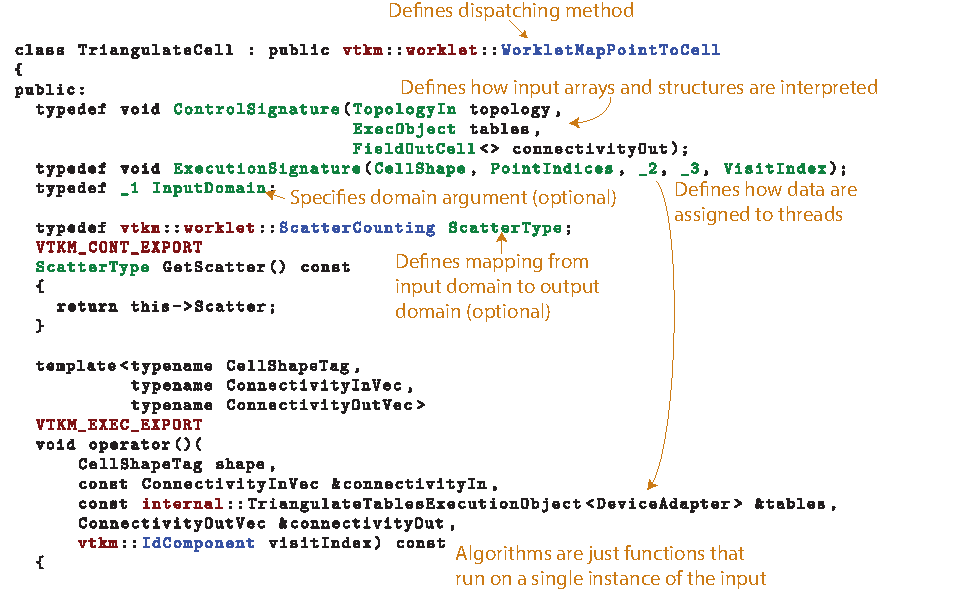
\includegraphics[width=\linewidth]{images/WorkletExampleAnnotated}
  \caption{Annotated example of a worklet declaration.}
  \label{fig:WorkletExampleAnnotated}
\end{figure}

\subsection{Control Signature}
\label{sec:ControlSignature}

\index{control~signature|(}
\index{signature!control|(}
\index{worklet!control~signature|(}

The control signature of a worklet is the \textcode{typedef} of a function
prototype named \controlsignature. The function prototype matches the
calling specification used with the dispatcher invoke function.

The return type of the function prototype is always \textcode{void} because
the dispatcher invoke functions do not return values. The parameters of the
function prototype are \index{signature~tags}\keyterm{tags} that identify
the type of data that is expected to be passed to invoke. For example, a
\sigtag{FieldIn} tag declares that the worklet will operate on input field
data, typically held in a \vtkmcont{ArrayHandle} whereas a
\sigtag{TopologyIn} tag declares that the worklet will operate on a cell set
structure like those documented in Section~\ref{sec:DataSets:CellSets}.

Tags can also have modifiers on them, which are attached as template
parameters. For example, a \sigtag{FieldIn} tag has a template parameter
that allows you to specify what data types can be in the field. A
\sigtagmod{FieldIn}{Scalar} accepts only scalar values whereas
\sigtagmod{FieldIn}{Vec3} accepts only 3D vectors.

The signature tags and their modifiers are described in greater detail in
the following section on worklet types.

\subsubsection{Type List Tags}
\label{sec:TypeListTags}

\index{type~list~tags|(}
\index{control~signature!type~list~tags|(}

As stated previously, some \controlsignature tags have template parameters
that accept modifier tags. The most common type of modifier tag is a type
list to specify or restrict what types are valid with a particular
argument. For example, \sigtagmod{FieldIn}{Scalar} refers to an input field
of scalar values.

A type list tag can be any type list as described in
Section~\ref{sec:TypeLists}. For convenience, all worklet superclasses
define the following type list tags. You are not restricted to use these
tags, but they are the most convenient.

\begin{description}
\item[\sigtag{IdType}] A \vtkm{Id}.
\item[\sigtag{Id2Type}] A \vtkm{Id2}.
\item[\sigtag{Id3Type}] A \vtkm{Id3}.
\item[\sigtag{IdComponentType}] A \vtkm{IdComponent}.
\item[\sigtag{Index}] A type used for indexing. Specifically \vtkm{Id},
  \vtkm{Id2}, or \vtkm{Id3}.
\item[\sigtag{Scalar}] A type used for scalar fields. Specifically
  \vtkm{Float32} or \vtkm{Float64}.
\item[\sigtag{Vec2}] A \vtkm{Vec} type of size two containing floating
  point numbers. Specifically
  \vtkm{Vec}\textcode{<}\vtkm{Float32}\textcode{,2>} and
  \vtkm{Vec}\textcode{<}\vtkm{Float64}\textcode{,2>}.
\item[\sigtag{Vec3}] A \vtkm{Vec} type of size three containing floating
  point numbers.
\item[\sigtag{Vec4}] A \vtkm{Vec} type of size four containing floating
  point numbers.
\item[\sigtag{FieldCommon}] A type commonly used in fields. Specifically
  anything in \sigtag{Scalar}, \sigtag{Vec2}, \sigtag{Vec3}, or
  \sigtag{Vec4}.
\item[\sigtag{VecCommon}] Any commonly used vector. Specifically, this is
  any vector of size 2, 3, or 4 that has components of type \vtkm{UInt8},
  \vtkm{Int32}, \vtkm{Int64}, \vtkm{Float32}, or \vtkm{Float64}.
\item[\sigtag{VecAll}] A vector of two, three, or four components
  containing any float or integer type.
\item[\sigtag{AllTypes}] Any possible type.
\end{description}

\index{control~signature!type~list~tags|)}
\index{type~list~tags|)}

\index{worklet!control~signature|)}
\index{signature!control|)}
\index{control~signature|)}

\subsection{Execution Signature}
\label{sec:ExecutionSignature}

\index{execution~signature|(}
\index{signature!execution|(}
\index{worklet!execution~signature|(}

Like the control signature, the execution signature of a worklet is the
\textcode{typedef} of a function prototype named \executionsignature. The
function prototype must match the parenthesis operator in terms of arity
and argument semantics.

The arguments of the \executionsignature's function prototype are tags that
define where the data come from. The most common tags are an underscore
followed by a number, such as \sigtagnum{1}, \sigtagnum{2}, etc. These
numbers refer back to the corresponding argument in the
\controlsignature. For example, \sigtagnum{1} means data from the first
control signature argument, \sigtagnum{2} means data from the second
control signature argument, etc.

Unlike the control signature, the execution signature optionally can
declare a return type if the parenthesis operator returns a value. If this
is the case, the return value should be one of the numeric tags
(i.e. \sigtagnum{1}, \sigtagnum{2}, etc.) to refer to one of the data
structures of the control signature. If the parenthesis operator does not
return a value, then \executionsignature should declare the return type as
\textcode{void}.

In addition to the numeric tags, there are other execution signature tags
to represent other types of data. For example, the \sigtag{WorkIndex} tag
identifies the instance of the worklet invocation. Each call to the worklet
function will have a unique \sigtag{WorkIndex}. Other such tags exist and
are described in the following section on worklet types where appropriate.

\index{worklet!execution~signature|)}
\index{signature!execution|)}
\index{execution~signature|)}

\subsection{Input Domain}
\label{sec:InputDomain}

\index{input~domain|(}
\index{worklet!input~domain|(}

Every worklet has one input argument in the \controlsignature identified as
its input domain. When a dispatcher invokes a worklet, it uses the input
argument to determine how many instances of the worklet to run.

Different types of worklets can have different types of domain. For example
a simple field map worklet has a \sigtag{FieldIn} argument as its input
domain, and the size of the input domain is taken from the size of the
associated field array. Likewise, a worklet that maps topology has a
\sigtag{TopologyIn} argument as its input domain, and the size of the input
domain is taken from the cell set.

A worklet specifies its input domain by creating a \textcode{typedef} named
\sigtag{InputDomain}. The object used in the \textcode{typedef} should be
one of the numeric tags (i.e. \sigtagnum{1}, \sigtagnum{2}, etc.) that
points to the appropriate \controlsignature argument.

Specifying the \sigtag{InputDomain} is optional. If it is not specified,
the first argument is assumed to be the input domain.

\index{worklet!input~domain|)}
\index{input~domain|)}

\subsection{Worklet Types}
\label{sec:WorkletTypes}

\index{worklet~types|(}

There are multiple worklet types provided by VTK-m, each designed to
support a particular type of operation. This section describes each of the
worklet types, identifies the generic superclass that a worklet instance
should derive, lists the signature tags and their meanings, and gives an
example of the worklet in use.

\newcommand{\commoncontrolsignaturetags}{
\item[\sigtag{WholeArrayIn}] This tag represents an array where all entries
  can be read by every worklet invocation. A \sigtag{WholeArrayIn} argument
  expects an \textidentifier{ArrayHandle} in the associated parameter of
  the dispatcher's \textcode{Invoke}. An array portal capable of reading
  from any place in the array is given to the worklet. Whole arrays are
  discussed in detail in Section~\ref{sec:WholeArrays} starting on
  page~\pageref{sec:WholeArrays}.

\item[\sigtag{WholeArrayOut}] This tag represents an array where any entry
  can be written by any worklet invocation. A \sigtag{WholeArrayOut}
  argument expects an \textidentifier{ArrayHandle} in the associated
  parameter of the dispatcher's \textcode{Invoke}. An array portal capable
  of writing to any place in the array is given to the worklet. Developers
  should take care when using writable whole arrays as introducing race
  conditions is possible. Whole arrays are discussed in detail in
  Section~\ref{sec:WholeArrays} starting on page~\pageref{sec:WholeArrays}.

\item[\sigtag{WholeArrayInOut}] This tag represents an array where any
  entry can be read or written by any worklet invocation. A
  \sigtag{WholeArrayInOut} argument expects an \textidentifier{ArrayHandle}
  in the associated parameter of the dispatcher's \textcode{Invoke}. An
  array portal capable of reading from or writing to any place in the array
  is given to the worklet. Developers should take care when using writable
  whole arrays as introducing race conditions is possible. Whole arrays are
  discussed in detail in Section~\ref{sec:WholeArrays} starting on
  page~\pageref{sec:WholeArrays}.

\item[\sigtag{ExecObject}] This tag represents an execution object that is
  passed directly from the control environment to the worklet. A
  \sigtag{ExecObject} argument expects a subclass of
  \vtkmexec{ExecutionObjectBase}, and this same object is given to the
  worklet. Execution objects are discussed in detail in
  Section~\ref{sec:ExecutionObjects} starting on
  page~\pageref{sec:ExecutionObjects}.
}

\newcommand{\numericexecutionsignaturetags}{
\item[\sigtagnum{1}, \sigtagnum{2},$\ldots$] These reference the
  corresponding parameter in the \controlsignature.
}

\newcommand{\commonexecutionsignaturetags}{
\item[\sigtag{WorkIndex}] This tag produces a \vtkm{Id} that uniquely
  identifies the invocation of the worklet.
\item[\sigtag{VisitIndex}] This tag produces a \vtkm{IdComponent} that
  uniquely identifies when multiple worklet invocations operate on the same
  input item, which can happen when defining a worklet with scatter (as
  described in Section~\ref{sec:WorkletScatter}).
}

\subsubsection{Field Map}
\label{sec:WorkletMapField}

\index{worklet~types!field~map|(}
\index{field~map~worklet|(}
\index{map~field|(}

A worklet deriving \vtkmworklet{WorkletMapField} performs a basic mapping
operation that applies a function (the operator in the worklet) on all the
field values at a single point or cell and creates a new field value at
that same location. Although the intention is to operate on some variable
over a mesh, a \vtkmworklet{WorkletMapField} may actually be applied to any
array.

A \textidentifier{WorkletMapField} subclass is invoked with a
\vtkmworklet{DispatcherMapField}. This dispatcher has two template
arguments. The first argument is the type of the worklet subclass. The
second argument, which is optional, is a device adapter tag.

A field map worklet supports the following tags in the parameters of its
\controlsignature.
\begin{description}
\item[\sigtag{FieldIn}] This tag represents an input field. A
  \sigtag{FieldIn} argument expects an \textidentifier{ArrayHandle} in the
  associated parameter of the dispatcher's \textcode{Invoke}. Each
  invocation of the worklet gets a single value out of this array.

  \sigtag{FieldIn} has a single template parameter that specifies what data
  types are acceptable for the array. The type tags are described in
  Section~\ref{sec:TypeListTags} starting on
  page~\pageref{sec:TypeListTags}.

  The worklet's \inputdomain can be set to a \sigtag{FieldIn} argument. In
  this case, the input domain will be the size of the array.

\item[\sigtag{FieldOut}] This tag represents an output field. A
  \sigtag{FieldOut} argument expects an \textidentifier{ArrayHandle} in the
  associated parameter of the dispatcher's \textcode{Invoke}. The array is
  resized before scheduling begins, and each invocation of the worklet sets
  a single value in the array.

  \sigtag{FieldOut} has a single template parameter that specifies what
  data types are acceptable for the array. The type tags are described in
  Section~\ref{sec:TypeListTags} starting on
  page~\pageref{sec:TypeListTags}.

\item[\sigtag{FieldInOut}] This tag represents field that is both an input
  and an output. A \sigtag{FieldInOut} argument expects an
  \textidentifier{ArrayHandle} in the associated parameter of the
  dispatcher's \textcode{Invoke}. Each invocation of the worklet gets a
  single value out of this array, which is replaced by the resulting value
  after the worklet completes.

  \sigtag{FieldInOut} has a single template parameter that specifies what
  data types are acceptable for the array. The type tags are described in
  Section~\ref{sec:TypeListTags} starting on
  page~\pageref{sec:TypeListTags}.

  The worklet's \inputdomain can be set to a \sigtag{FieldInOut} argument. In
  this case, the input domain will be the size of the array.

  \commoncontrolsignaturetags
\end{description}

A field map worklet supports the following tags in the parameters of its
\executionsignature.
\begin{description}
  \numericexecutionsignaturetags

  \commonexecutionsignaturetags
\end{description}

\index{map~field|)}
\index{field~map~worklet|)}
\index{worklet~types!field~map|)}

\subsubsection{Topology Map}
\label{sec:WorkletMapTopology}

\index{worklet~types!topology~map|(}
\index{topology~map~worklet|(}
\index{map~topology|(}

\index{map~topology|)}
\index{topology~map~worklet|)}
\index{worklet~types!topology~map|)}

\subsubsection{Point to Cell Map}
\label{sec:WorkletMapPointToCell}

\index{worklet~types!point~to~cell~map|(}
\index{point~to~cell~map~worklet|(}
\index{map~point~to~cell|(}

\index{map~point~to~cell|)}
\index{point~to~cell~map~worklet|)}
\index{worklet~types!point~to~cell~map|)}

\fix{When is cell to point map going to be implemented?}

%% \subsubsection{Cell to Point Map}
%% \label{sec:WorkletMapCellToPoint}

%% \index{worklet~types!cell~to~point~map|(}
%% \index{cell~to~point~map~worklet|(}
%% \index{map~cell~to~point|(}

%% \index{map~cell~to~point|)}
%% \index{cell~to~point~map~worklet|)}
%% \index{worklet~types!cell~to~point~map|)}

\index{worklet~types|)}

\subsection{WholeArrays}
\label{sec:WholeArrays}

\index{whole~array|(}
\index{worklet!whole~array|(}
\index{control~signature!whole~array|(}

\index{control~signature!whole~array|)}
\index{worklet!whole~array|)}
\index{whole~array|)}

\subsection{Execution Objects}
\label{sec:ExecutionObjects}

\index{execution~object|(}
\index{worklet!execution~object|(}
\index{control~signature!execution~object|(}

\index{control~signature!execution~object|)}
\index{worklet!execution~object|)}
\index{execution~object|)}

\subsection{Scatter}
\label{sec:WorkletScatter}

\index{scatter|(}
\index{worklet!scatter|(}

\fix{Don't forget scatters.}

\index{worklet!scatter|)}
\index{scatter|)}

\index{worklet!creating|)}
\index{worklet|)}

\section{Error Handling}
\label{sec:ExecutionEnvironment:ErrorHandling}

\section{Math}


\section{Working with Topology}

In the control environment, data is defined in mesh structures that
comprise a set of finite cells. (See Section~\ref{sec:DataSets:CellSets}
starting on page~\pageref{sec:DataSets:CellSets} for information on
defining cell sets in the control environment.) When worklets that operate
on cells are scheduled, these grid structures are broken into their
independent cells, and that data is handed to the worklet. Thus, cell-based
operations in the execution environment exclusively operate on independent
cells.

Unlike some other libraries such as VTK, VTK-m does not have a cell class
that holds all the information pertaining to a cell of a particular type.
Instead, VTK-m provides tags or identifiers defining the cell shape, and
companion data like coordinate and field information are held in separate
structures. This organization is designed so a worklet may specify exactly
what information it needs, and only that information will be loaded.

\subsection{Cell Shape Tags and Ids}
\label{sec:CellShapeTagsIds}

\index{shape|(}
\index{cell~shape|(}
\index{tag!cell~shape|(}
\index{tag!shape|(}

Cell shapes can be specified with either a tag (defined with a struct with
a name like \textidentifier{CellShapeTag*}) or an enumerated identifier
(defined with a constant number with a name like
\textidentifier{CELL\_SHAPE\_*}). These shape tags and identifiers are
defined in \vtkmheader{vtkm}{CellShape.h} and declared in the \vtkm{}
namespace (because they can be used in either the control or the execution
environment). Figure~\ref{fig:CellShapes} gives both the identifier and the
tag names.

\begin{figure}
  \centering
  \small
  \begin{tabular}{@{}c@{~}c@{~}c@{}}
    \raisebox{-0.5\height}{
\includegraphics{images/CellConnectionsVertex}} &
    \raisebox{-0.5\height}{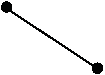
\includegraphics{images/CellConnectionsLine}} &
    \raisebox{-0.5\height}{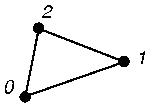
\includegraphics{images/CellConnectionsTriangle}} \\
    \vtkm{CELL\_SHAPE\_VERTEX} &
    \vtkm{CELL\_SHAPE\_LINE} &
    \vtkm{CELL\_SHAPE\_TRIANGLE} \\
    \vtkm{CellShapeTagVertex} \index{vertex} &
    \vtkm{CellShapeTagLine} \index{line} &
    \vtkm{CellShapeTagTriangle} \index{triangle} \\[2ex]
    \raisebox{-0.5\height}{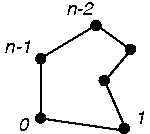
\includegraphics{images/CellConnectionsPolygon}} &
    \raisebox{-0.5\height}{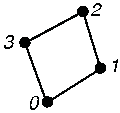
\includegraphics{images/CellConnectionsQuadrilateral}} &
    \raisebox{-0.5\height}{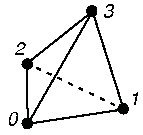
\includegraphics{images/CellConnectionsTetrahedron}} \\
    \vtkm{CELL\_SHAPE\_POLYGON} &
    \vtkm{CELL\_SHAPE\_QUAD} &
    \vtkm{CELL\_SHAPE\_TETRA} \\
    \vtkm{CellShapeTagPolygon} \index{polygon} &
    \vtkm{CellShapeTagQuad} \index{quadrilateral} &
    \vtkm{CellShapeTagTetra} \index{tetrahedron} \\[2ex]
    \raisebox{-0.5\height}{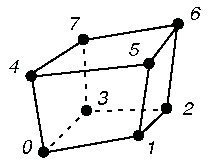
\includegraphics{images/CellConnectionsHexahedron}} &
    \raisebox{-0.5\height}{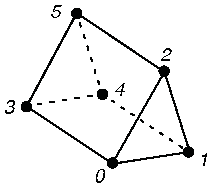
\includegraphics{images/CellConnectionsWedge}} &
    \raisebox{-0.5\height}{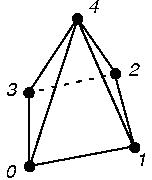
\includegraphics{images/CellConnectionsPyramid}} \\
    \vtkm{CELL\_SHAPE\_HEXAHEDRON} &
    \vtkm{CELL\_SHAPE\_WEDGE} &
    \vtkm{CELL\_SHAPE\_PYRAMID} \\
    \vtkm{CellShapeTagHexahedron} \index{hexahedron} &
    \vtkm{CellShapeTagWedge} \index{wedge} &
    \vtkm{CellShapeTagPyramid} \index{pyramid}
  \end{tabular}
  \caption{Basic Cell Shapes}
  \label{fig:CellShapes}
\end{figure}

In addition to the basic cell shapes, there is a special ``empty'' cell
with the identifier \vtkm{CELL\_SHAPE\_EMPTY} and tag
\vtkm{CellShapeTagEmpty}. This type of cell has no points, edges, or faces
and can be thought of as a placeholder for a null or void cell.

There is also a special cell shape ``tag'' named \vtkm{CellShapeTagGeneric}
that is used when the actual cell shape is not known at compile time.
\textidentifier{CellShapeTagGeneric} actually has a member variable named
\textcode{Id} that stores the identifier for the cell shape. There is no
equivalent identifier for a generic cell; cell shape identifiers can be
placed in a \vtkm{IdComponent} at runtime.

\fix{Add other basic cell shape features such as traits, converting back
  and forth, and \vtkmmacro{vtkmGenericCellShapeMacro}.}

\index{tag!shape|)}
\index{tag!cell~shape|)}
\index{cell~shape|)}
\index{shape|)}

\subsection{Parametric and World Coordinates}

\subsection{Interpolation}

\subsection{Derivatives}
